\chapter{{Introduction}}

\section{Modelos}

\subsection{Tabela}

%How to insert a table

COMO INSERIR UMA TABELA:

\begin{table}[ptbh]
\caption{Varia\c{c}\~{a}o de temperatura, para trajet\'{o}ria 2, ao longo da
simula\c{c}\~{a}o de din\^{a}mica molecular para diferentes modelos e
\textit{ensembles}.}%
\label{Tabela 02}
\begin{center}%
\begin{tabular}
[c]{c|c|c|c|c}\hline\hline
\multicolumn{5}{c}{\textbf{Trajet\'{o}ria 2}}\\\hline
\textit{Ensemble/}\textbf{Modelo} & \textbf{In\'{\i}cio} & \textbf{M\'{a}ximo}
& \textbf{M\'{\i}nimo} & \textbf{Estabiliza\c{c}\~{a}o}\\\hline\hline
\multicolumn{1}{l|}{\textbf{NVT/SPC}} & 299,350 & 300,125 & 299,825 &
10ps\\\hline
\multicolumn{1}{l|}{\textbf{NVT/SPCE}} & 299,640 & 300,050 & 299,920 &
19ps\\\hline
\multicolumn{1}{l|}{\textbf{NPT/SPC}} & 299,730 & 300,080 & 299,835 &
08ps\\\hline
\multicolumn{1}{l|}{\textbf{NPT/SPCE}} & 300,650 & 300,050 & 299,850 &
06ps\\\hline\hline
\end{tabular}
\newline
\end{center}
\end{table}


\subsection{Equa\c{c}\~{a}o}

%How to insert equation

COMO INSERIR UMA EQUA\c{C}\~{A}O:

\begin{equation}
V_{LJ}=-\left(  \frac{A}{r}\right)  ^{6}+\left(  \frac{B}{r}\right)  ^{12}
\label{Eq LJ}%
\end{equation}
\newpage


\subsection{Figuras}

%How to insert diferent kinds of graphics file

COMO INSERIR FIGURAS:

Testing with .png file especification:\\
\begin{figure}[htbp]
  \begin{center}
    \includegraphics
    {figures/lncc.png}
    \caption{A .png picture.}
    \label{Figura}
  \end{center}
\end{figure}
%\newpage

Testing with .eps file converted from .pdf (without extension file
especification) by ./pdfcompila, and with resize figure by tex comand $\backslash$resizebox\{Xcm\}\{!\}:
\begin{figure}[htbp]
  \begin{center}
    \resizebox{9cm}{!}{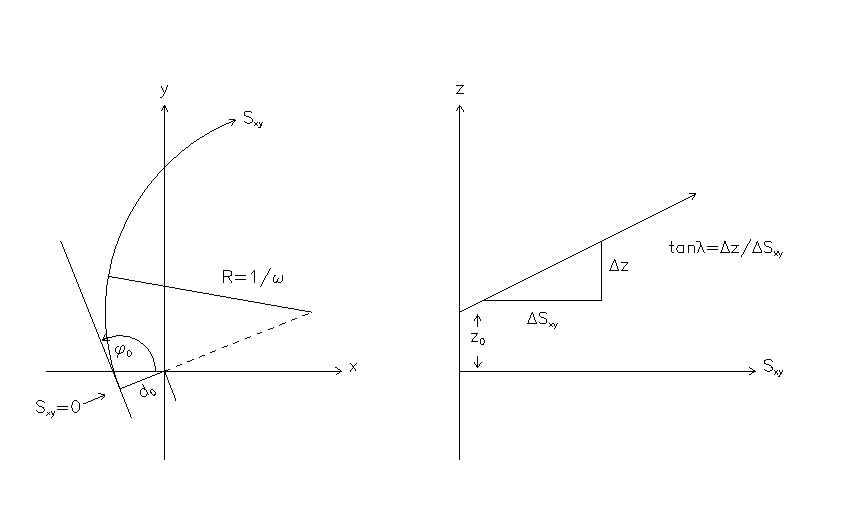
\includegraphics
    {figures/helix}}
    \caption{A resized .eps figure.}
    \label{Figura 0}
  \end{center}
\end{figure}
%\newpage

Testing include graphics with many extension files without type any
extension in tex file. Here was utilized other way to resize figure
(by setting original size and aim size):
\begin{figure}[htbp]
  \begin{center}
    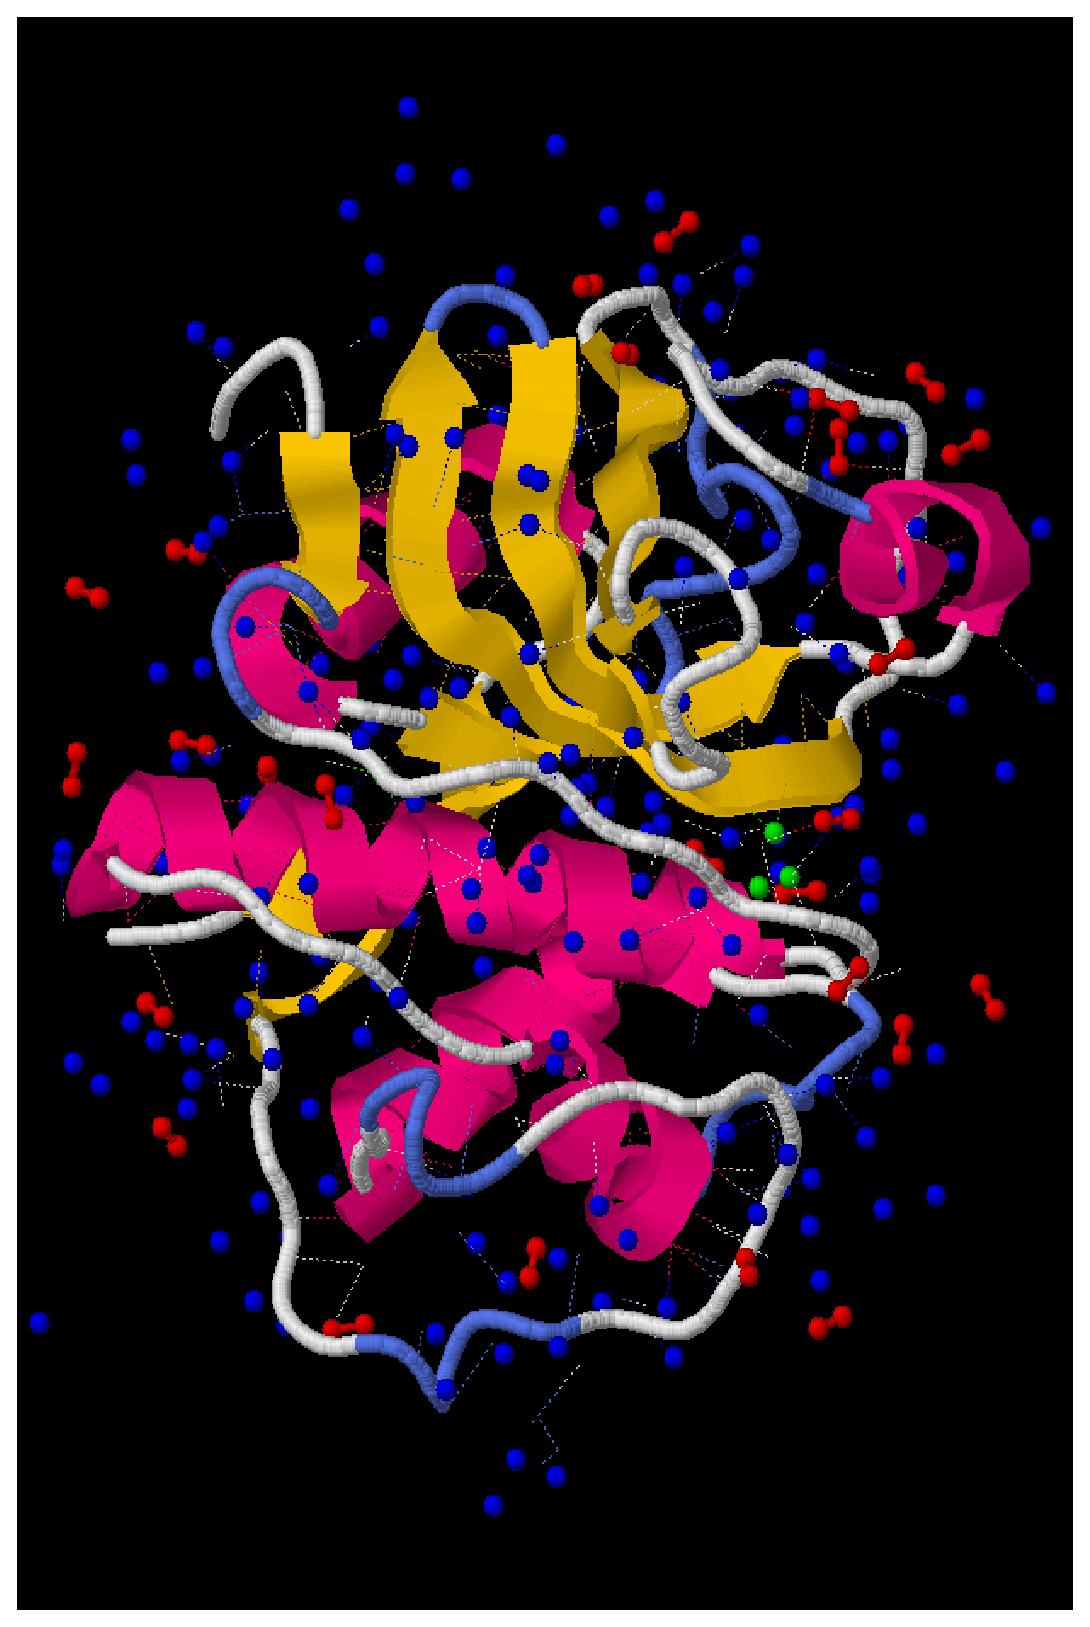
\includegraphics
    [natheight=7.050000in,
      natwidth=10.630300in,
      height=2.0588in,
      width=3.5982in]
    {figures/9pap}
    \caption{A colourful picture.}
    \label{Figura 01}
  \end{center}
\end{figure}
\newpage

This is how you refer to the figure in the text:
The picture in Figure~\ref{Figura} is grayscale and Figure~\ref{Figura
  0} and  Figure~\ref{Figura 01} is colourful.


\section{Cita\c{c}\~{a}o e Refer\^{e}ncia}

COMO INSERIR REFER\^ENCIAS BIBLIOGR\'AFICAS:

References should be cited in the text by name (year) or
(name, year). For example:

"In a classical work, \citet{ANENPI2006} proposed ...," (\textbf{one author})% For one author

or

"In a recent work \citep{Altschul1990}, it was proposed ..." (\textbf{more than two authors})
\\
In this case use
the commands $\backslash$cite or $\backslash$citet and $\backslash$citep for citations.
\\

%How to insert references
- Examples to how insert direct reference/citation:

"According to \cite{Altschul1990} ..." \textbf{(more than two authors)  ($\backslash$cite)} % For multiple authors

or

"According to \citet{Coura2002} ..." \textbf{(two authors) ($\backslash$citet)} % For multiple authors
\\

- Examples to how insert indirect reference/citation \cite{GOLDBERG}:

"In a recent work \citep{Altschul1990}, it was proposed ..." \textbf{(more than two authors)  ($\backslash$citep)} % For multiple authors

or

"In a recent work \citep{Coura2002}, it was proposed ..." \textbf{(two authors)  ($\backslash$citep)} % For two authors
\\

References will be listed in alphabetical order at the end of the paper. Each reference must be cited in the text.

Format of references (see these examples in index):
\begin{itemize}
\item Article: \cite{Altschul1990}.
\item Unpublished Article: \cite{ANENPI2006}.
\item Book: \cite{BONABEAU}.
\item In Book: \cite{SILVEIRA}.
\item Incollection: \cite{MANIEZZO}.
\item Inproceedings: \cite{GOLDBERG}.
\item Master Thesis: \cite{Gomes2006}.
\item Doctor and PhD Thesis: \cite{Rossle2004}.
\item Technical Report: \cite{WHO2002}.
\item Miscellaneous: \cite{CORUS05}.

\item TESTE: \cite{Berkhin2006}
\item TESTE: \cite{Kogan2006}



\end{itemize}
